\section{The Machine}

In some sense, particle physicists conduct high energy physics experiments in an unimaginative way. To study what is inside the proton we accelerate them to very high speed and smash them together to see what comes out. The searches of Higgs boson for instance relies heavily on accelerators which have high enough center of mass energy to produce them. The Large Hadron Collider is the largest physics experiment ever constructed in the history of mankind. The designed maximum center of energy can reach 14\tev. The cancellation of the US super-conducting super-collider made the LHC the most powerful accelerator in the world. Within the forseable future (in a scale of 10 years), as no country has expressed explicit interest in constructing the next collider, the LHC will retian this title for a long time. As the US has terminated the operation of the Tevatron, the LHC is also the only machine with which the Higgs boson can be studied at the moment.

The LHC is located across the boarder between Switzerland and France. It is one of the accelerators of the acclerator complex at the European Organization for Nuclear Research (CERN) Fig.\ref{fig:lhc-CERN} located in Geneva, Switzerland. The tunnel of the LHC is 27 km in circumference and 100 meters underground. Before the LHC era, the tunnel was used to host an electron-positron collider called LEP\cite{refneeded}. Two beams of particles go around the accelerator in opposite directions and cross each other at four interaction locations where the four experiments ATLAS, CMS, ALICE and LHCb are located. Proton-proton collision is the main usage of the LHC, while usually during the last few weeks of operations of each year the machine also collide heavy ions.

\begin{figure}[htpb!]
\begin{center}
  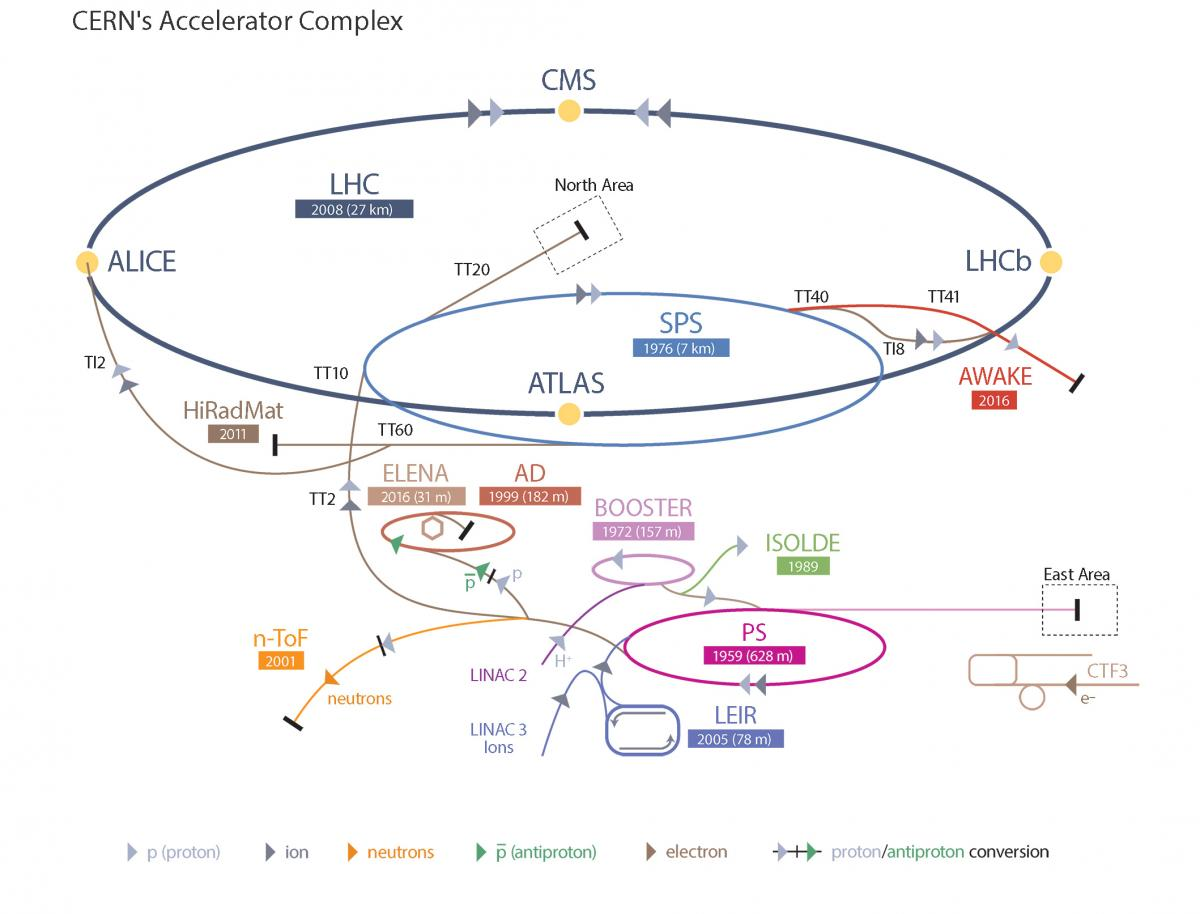
\includegraphics[width=0.7\linewidth]{figures/LHC/LHC_default}
\caption{Diagram of the CERN Accelerator Complex}
\label{fig:lhc-CERN}
\end{center}
\end{figure}


Acceleration of the protons are staged. Many smaller accelerators historically built for lower energy experiments are utilized to pre-accelerate the beams before injecting them to the LHC. We obtain the protons from hydrogen gass and first put them through the very first linear accelerator Linac2. The outcoming protons are accelerated to 50\mev and enter a small ring accelerator of radius 25 meters called Proton Synchrotron Booster to be accelerated up to 1.4\gev. Then the protons are fed into the Proton Synchrotron, 100 meters in radius, and accelerated to 25\gev. The Super Proton Synchrotron of radius 6.9 kilo-meters then accelerate the beams to 450\gev and eventually inject the beams into the LHC. The LHC depending on its configuration can evetually accelerate the beams to 7 to 14\tev.

Radio Frequency (RF) cavities are usd by the LHC to accelerate particles. Each of the LHC beam has 8 RF cavities, each of which delivers 2MV acceleration to the partiles. The frequency of the RF cavities are held at 400$MHz$ which is an integer multiple (called harmonic number $\approx$ 35600)of the revolution frequency $f$ of the protom beam so that the protons of right energies are not accelerated anymore. To bend the protons inside the circular accelerator, super-conducting magnetic dipoles are used. The collision energy is directly proportional to the dipole field strength. For a 13\tev collider, the dipole field strength needed is about 8.33 telsa. The LHC employs in total 1232 dipoles which are built with NbTi coils which needed to be cooled for weeks down to 1.9$K$ with Helium to reach super-conductivity.

Most of the collision at the LHC are boring QCD events and only with very small probabilities are we able to produce interesting partiles such as Higgs \ref{fig:lhc-lhccrossection}. Therefore, we need to collide as many pairs of protons as possible to accumulate sufficient statistics. The beams at the LHC contains proton bunches which are spaced at 25ns. The nominal proton beams in LHC come with 2808 bunches with each bunch containing $1.15\times 10^{11}$ protons with the beam size being 3.5 micrometers. Since 2016, the filling scheme of the LHC changed to Batch Compression Merging and Splitting (BCMS) and reduced the number of bunches down to 2556 per ring while reducing the beam size down to 2.5 micrometers and retaining $1.15\times 10^{11}$ protons per bunch. As the LHC delivers round symmetric beams, this change yielded brighter beams by lowering the bunch emittance in the instantaneous luminosity equation\ref{eq:lumi}. In Eq.\ref{eq:lumi}, N is the number of protons per bunch, $n_c$ is the number of crossing bunches, f is the beam revolution frequency, $\gamma$ is the relativistic factor, $\epsilon_n$ is the normalized emittance, $\beta_{\text{ip}}$ is the beta function value at the interaction point and the F factor corrects for luminosity loss due to cross angle. The average number of interactions per bunch crossing at the Interaction Point 1 for the ATLAS experiment from 2015 to 2018 was measured to be $<\mu>=34.2$\ref{fig:lhc-mu}. 


\begin{equation}
L = \frac{FN^2 n_c f\gamma}{4\pi \epsilon_n \beta_{\text{ip}}}
\label{eq:lumi}
\end{equation}


\begin{figure}[htpb!]
\begin{center}
  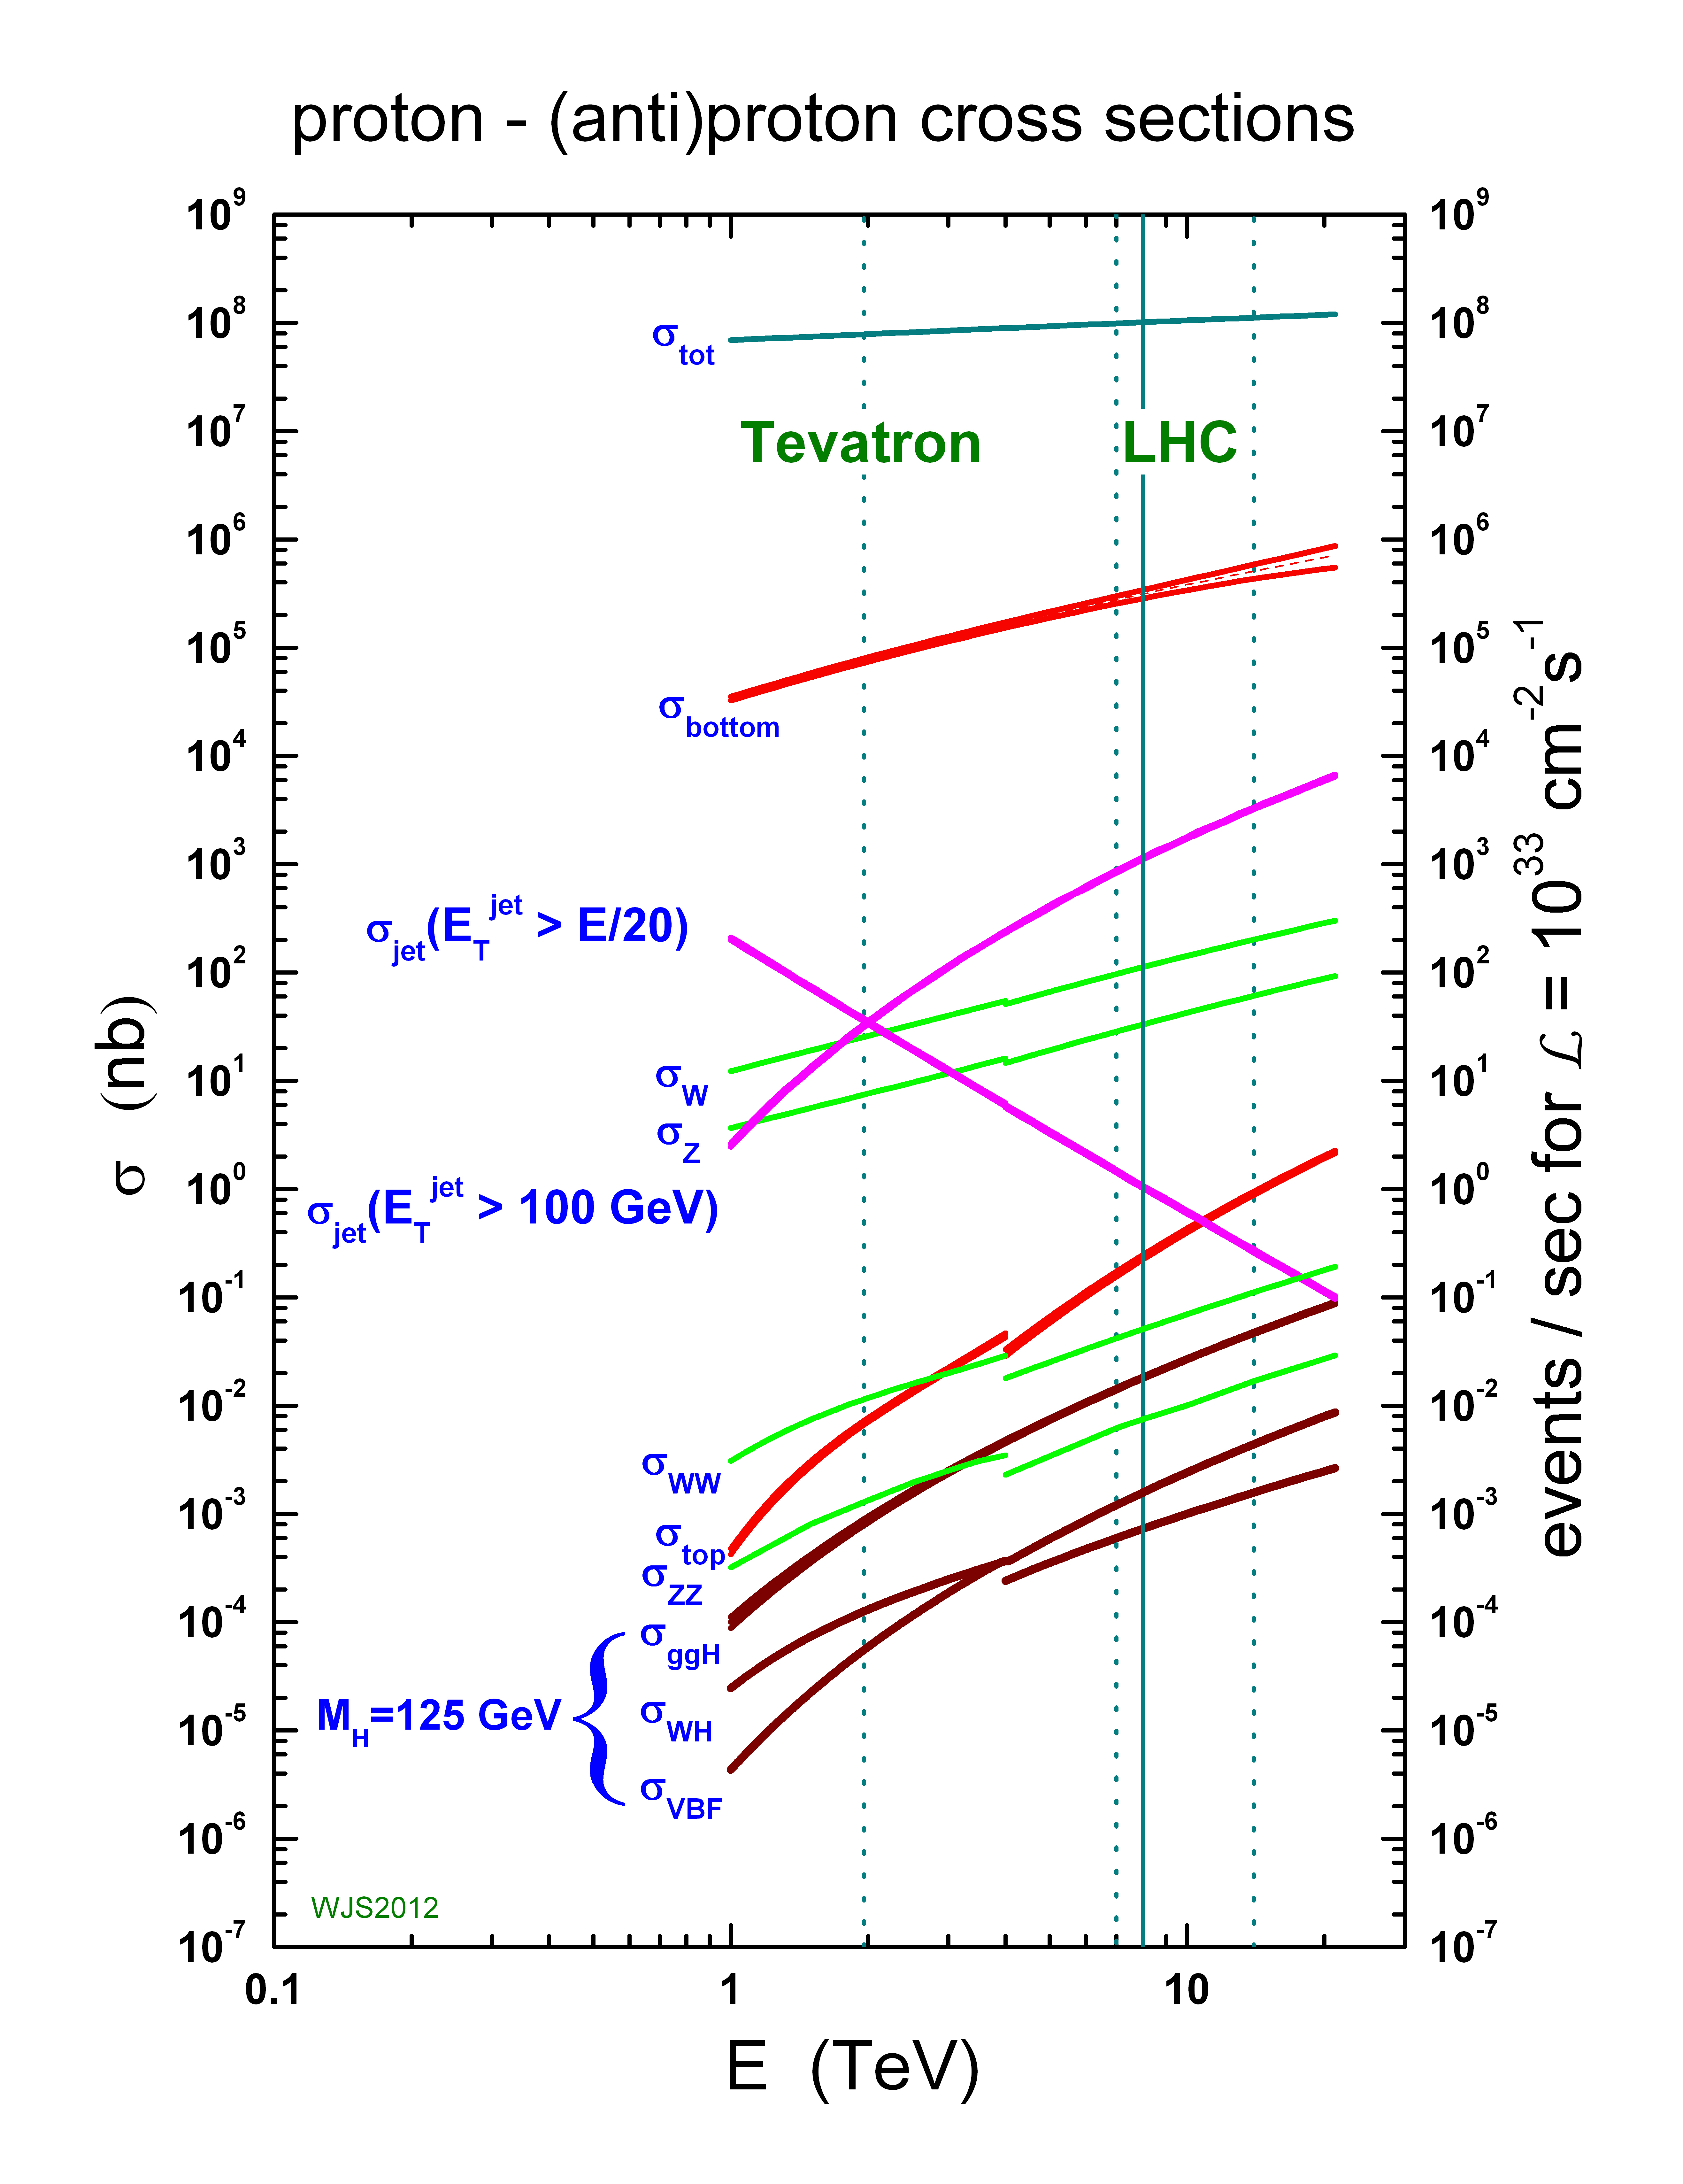
\includegraphics[width=0.6\linewidth]{figures/LHC/crosssections2013}
\caption{LHC Production Cross Sections}
\label{fig:lhc-lhccrossection}
\end{center}
\end{figure}

\begin{figure}[htpb!]
\begin{center}
  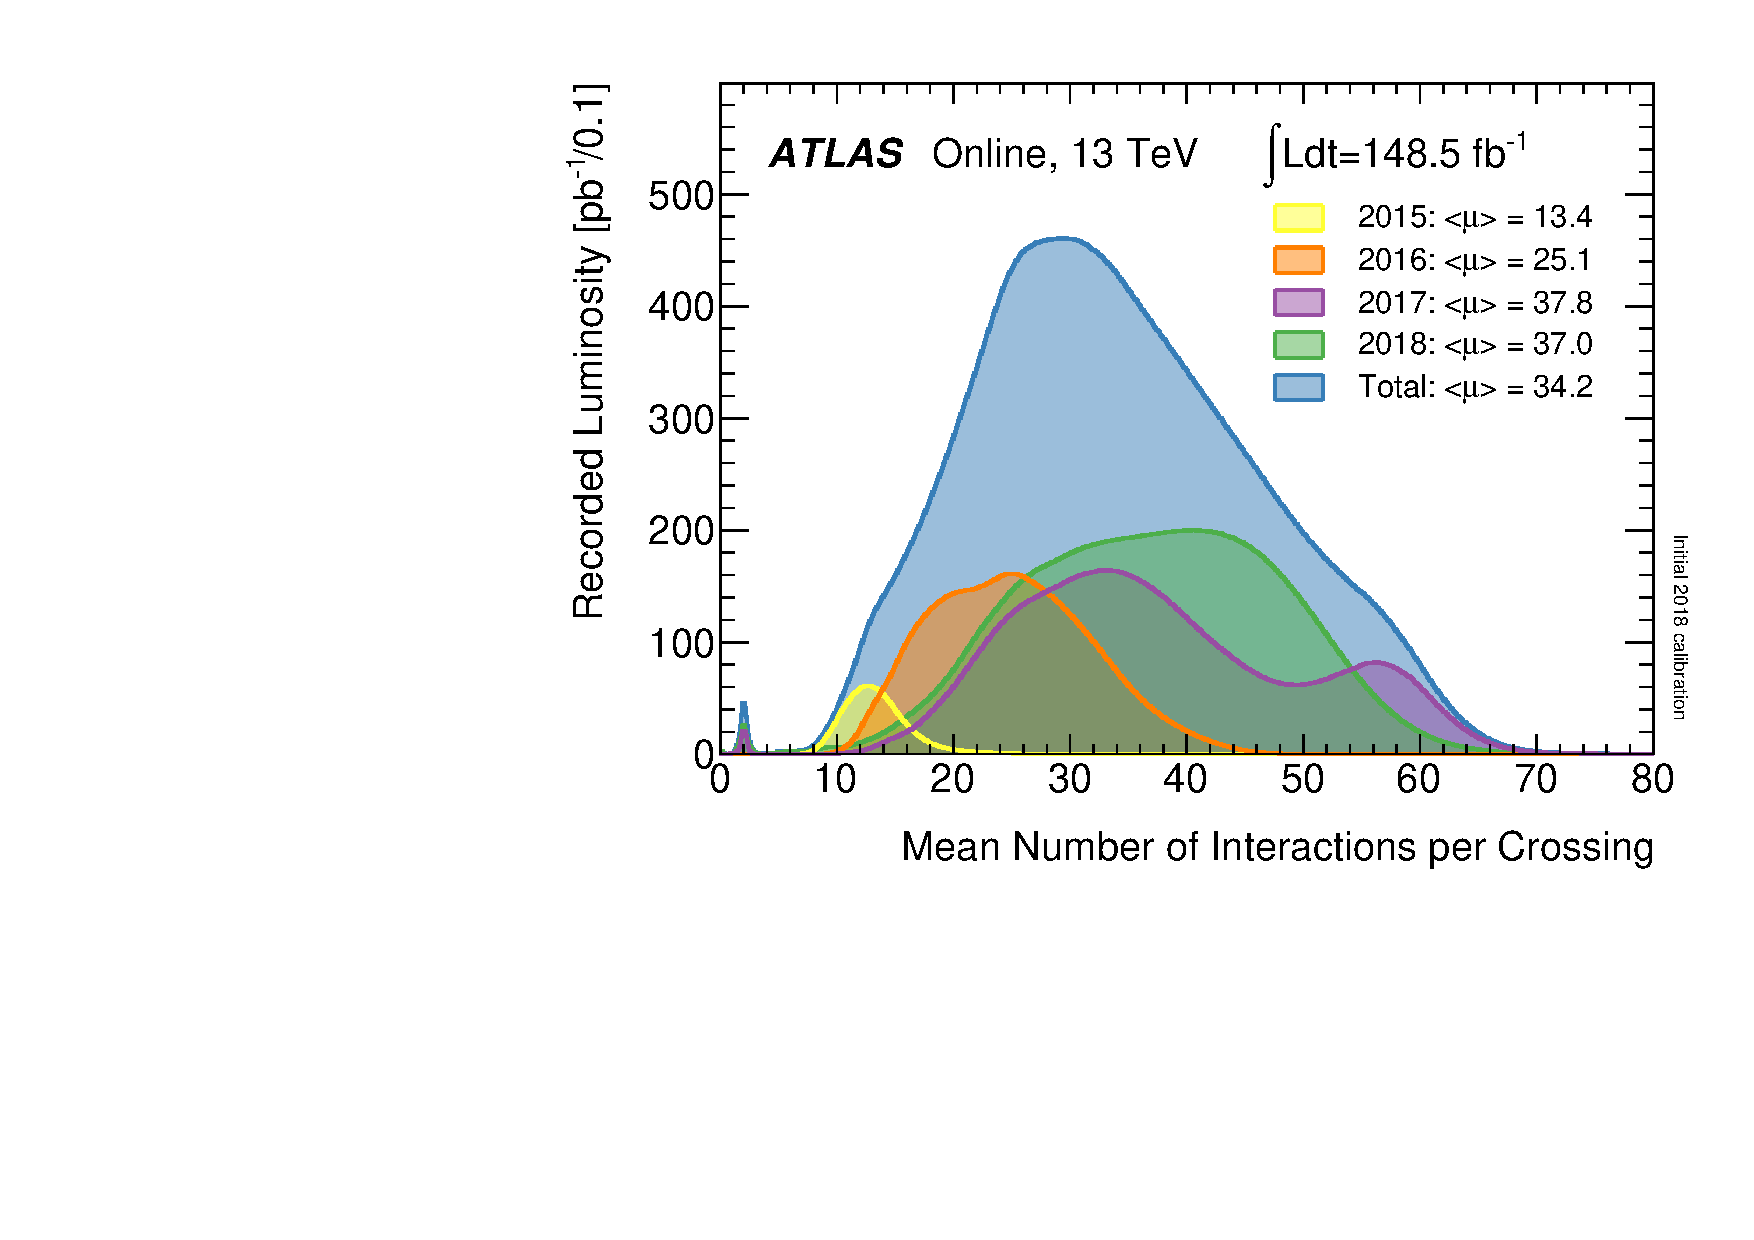
\includegraphics[width=0.6\linewidth]{figures/LHC/mu_2015_2018}
\caption{Number of interactions per bunch crossing}
\label{fig:lhc-mu}
\end{center}
\end{figure}

\section{Operations}

The LHC operation was planned for the tenure of the collider and so far has mostly stayed on track. The Run I experiments start in 2011. The energy of the collider will ramp up from 7 to 8\tev and deliver in total 30 \ifb. After the Long Shutdown from 2013 to 2014 (LS1), the machine restarted in 2015 with energy of 13\tev for Run II operation to deliver 150 \ifb of data. The machine is in the second long shutdown (LS2) and will restart in 2021 for Run III operation with 14\tev to deliver 300 \ifb of data. Eventually, after experiments upgrade, the LHC will enter HL-LHC era and keep running to deliver 3000\ifb of data. This thesis primarily uses the datasets collected during Run II LHC operation by the ATLAS detector. The luminosity accumulation through this period is shown in Fig.\ref{fig:lhc-lumi}. Specifically for the analyses used the 2016 dataset which amounts to 36 \ifb.


\begin{figure}[htpb!]
\begin{center}
  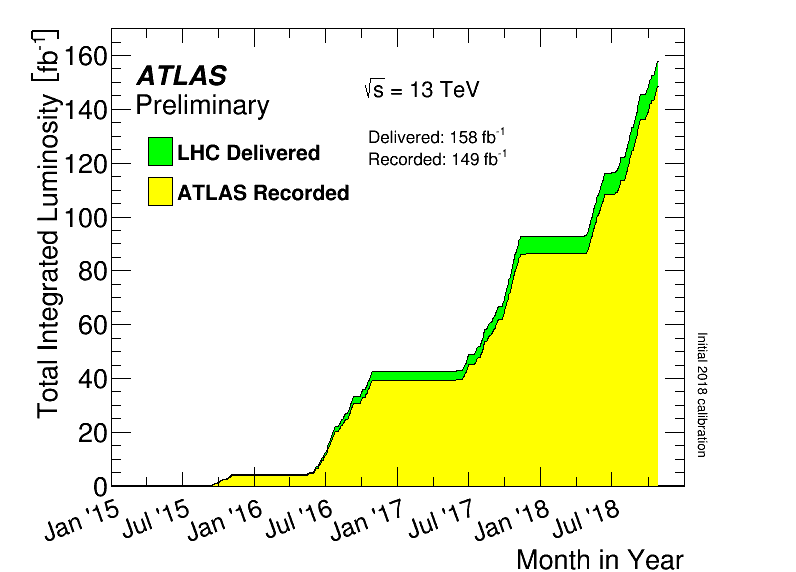
\includegraphics[width=0.5\linewidth]{figures/LHC/intlumivstimeRun2.png}
\caption{Integrated luminosity delivered by the LHC and collected by the ATLAS detector during the Run II experiment. The 2015 run was mostly a trial to test the collider and detector conditions after the LS1.}
\label{fig:lhc-lumi}
\end{center}
\end{figure}
